% Drawing 154/06-12 -- folder 154, batch 06, archive page 115 (PDF page 116).
% Transcription: page de dessins en couleur : sept demi-cercles vert clair aux extrémités marquées, certains arcs renforcés en brun ; dans trois d'entre eux, des droites rouges qui descendent du haut, verticales ou obliques, et de petits traits rouges sur le bord ; dans les trois de droite, le sommet marqué « $+1$ », les côtés marqués $\varepsilon_1$, $\varepsilon_2$, et des segments intérieurs au crayon portant $\varepsilon_1$, $\varepsilon_2$ et « $-1$ » ; en haut à droite, un cercle au crayon
% Kind: seven half-circles with marked ends, red lines and signs. Method 2 (schematic redraw from the facsimile). Status: partial.
% Notes: Page of colour drawings: seven light green half-circles with marked ends, some arcs reinforced in brown; in three of them red lines come down from the top, vertical or oblique, and small red strokes sit on the rim; in the three on the right the top is marked « +1 », the sides epsilon_1, epsilon_2, and pencil segments inside carry epsilon_1, epsilon_2 and « -1 »; a pencil circle top right. Read from the page view; the small red strokes on the rims are placed by groups. Still differs from the facsimile: see above.
% Coordinates: 1 unit = 1 mm = 1/100 of the crop width (bbox in page fractions: [0.211, 0.13, 0.909, 0.464]).
% Redrawn by Claude (claude-opus-5-5), issue #73, 2026-11-07; not checked by a human; not compiled (no TeX in the session).
% Revised by Claude (claude-opus-5-5) 2026-11-09 (issue #128) after Michel's check: vertices snapped to exact intersections (drawn points on their lines, meeting ends on the stroke they meet, near-concurrent lines through one computed point, curve ends on their rim); labels at \small as in folder 80 batch 3. Status: partial.
% Rights: reproduces part of the work -- behind RENDER_TRANSCRIPTS, never published by itself.
\documentclass[tikz,border=3pt]{standalone}
\usepackage{amsmath,amssymb}
\usetikzlibrary{patterns,arrows.meta}
\tikzset{Or/.style={orange!90!black}, Ye/.style={yellow!80!orange}, Lg/.style={green!60!black!70}, Dg/.style={green!45!black}, Br/.style={brown!80!black}, Rd/.style={red!85!black}, Bl/.style={blue!70!black}, Gy/.style={black!40}, pencil/.style={black!45}, struck/.style={black!35}, mark/.style={circle,draw,inner sep=1.3pt}, pt/.style={circle,fill,inner sep=0.9pt}, opt/.style={circle,draw,fill=white,inner sep=1.1pt}}
\begin{document}
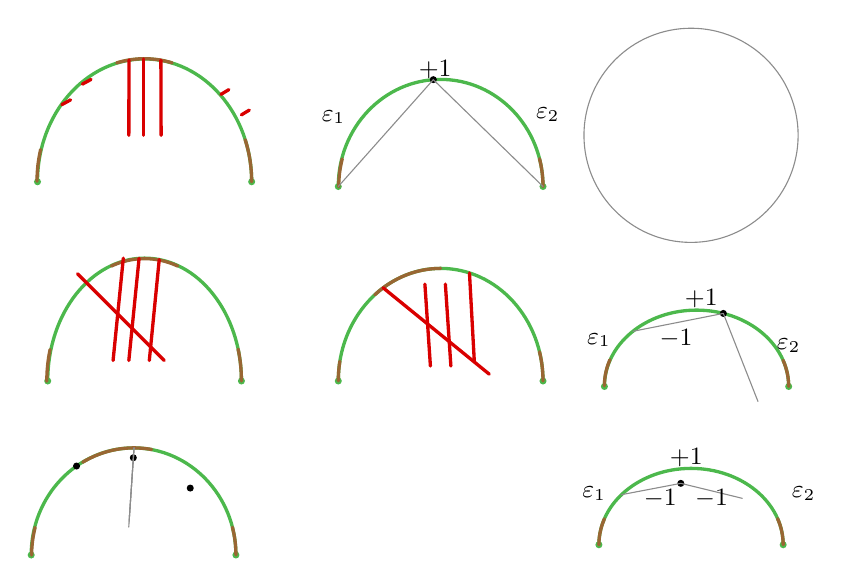
\begin{tikzpicture}[x=1mm,y=1mm,line cap=round,line join=round,font=\scriptsize]
\draw[Lg,very thick] (29.9,-18.2) arc[start angle=0, end angle=180, x radius=13.6, y radius=15.6];
\node[pt,Lg] at (2.7,-18.2) {};
\node[pt,Lg] at (29.9,-18.2) {};
\draw[Br,very thick] (3.1,-14.1) arc[start angle=165, end angle=180, x radius=13.6, y radius=15.6];
\draw[Br,very thick] (19.8,-3.1) arc[start angle=75, end angle=105, x radius=13.6, y radius=15.6];
\draw[Br,very thick] (29.9,-18.2) arc[start angle=0, end angle=20, x radius=13.6, y radius=15.6];
\draw[Rd,very thick] (14.32,-2.73) -- (14.3,-12.3);
\draw[Rd,very thick] (16.2,-2.6) -- (16.2,-12.3);
\draw[Rd,very thick] (18.37,-2.75) -- (18.4,-12.3);
\draw[Rd,very thick] (5.8,-8.4) -- (6.9,-7.8);
\draw[Rd,very thick] (8.4,-5.8) -- (9.5,-5.2);
\draw[Rd,very thick] (26,-7.1) -- (27,-6.5);
\draw[Rd,very thick] (28.6,-9.7) -- (29.6,-9.1);
\draw[Lg,very thick] (66.9,-18.8) arc[start angle=0, end angle=180, x radius=13, y radius=13.6];
\node[pt,Lg] at (40.9,-18.8) {};
\node[pt,Lg] at (66.9,-18.8) {};
\draw[Br,very thick] (41.4,-15.3) arc[start angle=165, end angle=180, x radius=13, y radius=13.6];
\draw[Br,very thick] (66.9,-18.8) arc[start angle=0, end angle=15, x radius=13, y radius=13.6];
\node[pt] at (52.97,-5.23) {};
\node[inner sep=1pt] at (53.2,-3.9) {\small $+1$};
\draw[pencil] (52.97,-5.23) -- (40.9,-18.8);
\draw[pencil] (52.97,-5.23) -- (66.9,-18.8);
\node[inner sep=1pt] at (40.3,-10) {\small $\varepsilon_1$};
\node[inner sep=1pt] at (67.5,-9.7) {\small $\varepsilon_2$};
\draw[pencil] (85.7,-12.3) circle[radius=13.6];
\draw[Lg,very thick] (28.6,-43.5) arc[start angle=0, end angle=180, x radius=12.3, y radius=15.6];
\node[pt,Lg] at (4,-43.5) {};
\node[pt,Lg] at (28.6,-43.5) {};
\draw[Br,very thick] (4.3,-39.5) arc[start angle=165, end angle=180, x radius=12.3, y radius=15.6];
\draw[Br,very thick] (20.5,-28.9) arc[start angle=70, end angle=110, x radius=12.3, y radius=15.6];
\draw[Br,very thick] (28.6,-43.5) arc[start angle=0, end angle=15, x radius=12.3, y radius=15.6];
\draw[Rd,very thick] (13.6,-27.9) -- (12.3,-40.9);
\draw[Rd,very thick] (15.6,-27.93) -- (14.3,-40.9);
\draw[Rd,very thick] (18.16,-28.08) -- (16.9,-40.9);
\draw[Rd,very thick] (7.8,-29.9) -- (18.8,-40.9);
\draw[Lg,very thick] (66.9,-43.5) arc[start angle=0, end angle=180, x radius=13, y radius=14.3];
\node[pt,Lg] at (40.9,-43.5) {};
\node[pt,Lg] at (66.9,-43.5) {};
\draw[Br,very thick] (41.1,-41) arc[start angle=170, end angle=180, x radius=13, y radius=14.3];
\draw[Br,very thick] (53.9,-29.2) arc[start angle=90, end angle=130, x radius=13, y radius=14.3];
\draw[Br,very thick] (66.9,-43.5) arc[start angle=0, end angle=15, x radius=13, y radius=14.3];
\draw[Rd,very thick] (51.9,-31.2) -- (52.6,-41.6);
\draw[Rd,very thick] (54.5,-31.2) -- (55.2,-41.6);
\draw[Rd,very thick] (57.56,-29.78) -- (58.18,-41.1);
\draw[Rd,very thick] (46.6,-31.67) -- (60.07,-42.63);
\draw[Lg,very thick] (98.1,-44.2) arc[start angle=0, end angle=180, x radius=11.7, y radius=9.7];
\node[pt,Lg] at (74.7,-44.2) {};
\node[pt,Lg] at (98.1,-44.2) {};
\draw[Br,very thick] (75.4,-40.8) arc[start angle=160, end angle=180, x radius=11.7, y radius=9.7];
\draw[Br,very thick] (98.1,-44.2) arc[start angle=0, end angle=20, x radius=11.7, y radius=9.7];
\node[pt] at (89.8,-34.92) {};
\node[inner sep=1pt] at (87,-33.1) {\small $+1$};
\draw[pencil] (78.32,-37.19) -- (89.8,-34.92) -- (94.2,-46.1);
\node[inner sep=1pt] at (74,-38.3) {\small $\varepsilon_1$};
\node[inner sep=1pt] at (98.1,-39) {\small $\varepsilon_2$};
\node[inner sep=1pt] at (83.8,-38.1) {\small $-1$};
\draw[Lg,very thick] (27.9,-65.6) arc[start angle=0, end angle=180, x radius=13, y radius=13.6];
\node[pt,Lg] at (1.9,-65.6) {};
\node[pt,Lg] at (27.9,-65.6) {};
\draw[Br,very thick] (2.4,-62.1) arc[start angle=165, end angle=180, x radius=13, y radius=13.6];
\draw[Br,very thick] (17.2,-52.2) arc[start angle=80, end angle=120, x radius=13, y radius=13.6];
\draw[Br,very thick] (27.9,-65.6) arc[start angle=0, end angle=15, x radius=13, y radius=13.6];
\node[pt] at (7.66,-54.3) {};
\node[pt] at (14.87,-53.25) {};
\node[pt] at (22.1,-57.1) {};
\draw[pencil] (14.96,-51.99) -- (14.29,-62.05);
\draw[pencil] (14.96,-51.99) -- (14.36,-60.97);
\draw[pencil] (14.96,-51.99) -- (14.33,-61.41);
\draw[Lg,very thick] (97.4,-64.3) arc[start angle=0, end angle=180, x radius=11.7, y radius=9.7];
\node[pt,Lg] at (74,-64.3) {};
\node[pt,Lg] at (97.4,-64.3) {};
\draw[Br,very thick] (74.7,-61) arc[start angle=160, end angle=180, x radius=11.7, y radius=9.7];
\draw[Br,very thick] (97.4,-64.3) arc[start angle=0, end angle=20, x radius=11.7, y radius=9.7];
\node[pt] at (84.4,-56.5) {};
\node[inner sep=1pt] at (85.1,-53.2) {\small $+1$};
\draw[pencil] (76.86,-57.94) -- (84.4,-56.5) -- (92.2,-58.4);
\node[inner sep=1pt] at (73.4,-57.8) {\small $\varepsilon_1$};
\node[inner sep=1pt] at (100,-57.8) {\small $\varepsilon_2$};
\node[inner sep=1pt] at (81.8,-58.4) {\small $-1$};
\node[inner sep=1pt] at (88.3,-58.4) {\small $-1$};
\end{tikzpicture}
\end{document}
